\documentclass[conference]{IEEEtran}
\IEEEoverridecommandlockouts
% The preceding line is only needed to identify funding in the first footnote. If that is unneeded, please comment it out.
\usepackage{cite}
\usepackage{amsmath,amssymb,amsfonts}
\usepackage{algorithmic}
\usepackage[ruled,vlined,linesnumbered]{algorithm2e}
\usepackage{graphicx}
\usepackage{textcomp}
\usepackage{xcolor}
\usepackage{flowchart}
\usetikzlibrary{shapes,arrows}
\def\BibTeX{{\rm B\kern-.05em{\sc i\kern-.025em b}\kern-.08em
    T\kern-.1667em\lower.7ex\hbox{E}\kern-.125emX}}
\begin{document}

\title{Detecting outliers in streaming time series data from ARM distributed sensors
%{\footnotesize \textsuperscript{*}Note: Sub-titles are not captured in Xplore and
%should not be used}
%\thanks{Identify applicable funding agency here. If none, delete this.}
}

\author{
\IEEEauthorblockN{Yuping Lu}
\IEEEauthorblockA{\textit{University of Tennessee}\\
Knoxville, TN, USA \\
yupinglu89@gmail.com}
\and
\IEEEauthorblockN{Nathan Collier}
\IEEEauthorblockA{\textit{Oak Ridge National Laboratory}\\
Oak Ridge, TN, USA \\
nathaniel.collier@gmail.com}
\and
\IEEEauthorblockN{Bhargavi Krishna}
\IEEEauthorblockA{\textit{Oak Ridge National Laboratory}\\
Oak Ridge, TN, USA \\
krishnab@ornl.gov}
\and
\IEEEauthorblockN{Michael A. Langston}
\IEEEauthorblockA{\textit{University of Tennessee}\\
Knoxville, TN, USA \\
langston@tennessee.edu}
\and
\IEEEauthorblockN{Jitendra Kumar}
\IEEEauthorblockA{\textit{Oak Ridge National Laboratory}\\
Oak Ridge, TN, USA \\
jkumar@climatemodeling.org}
}
\maketitle

%% Abstract
\begin{abstract}

The Atmospheric Radiation Measurement (ARM) Data Center at ORNL collects data
from a number of permanent and mobile facilities around the globe. The
data is then ingested to create high level scientific products. High
frequency streaming measurements from sensors and radar instruments at
ARM sites requires high degree of accuracy to enable rigorous study of
atmospheric processes. Outliers in collected data are common, however, 
due to instrument failure or extreme weather events. Thus, it is critical 
to identify and flag them. We employed multiple univariate, multivariate
and time series techniques for outlier detection methods and 
studied their effectiveness. First, we examined Pearson correlation coefficient 
which is used to measure the pairwise correlations between variables. 
Singular Spectrum Analysis (SSA) was applied to detect outliers by removing
the anticipated annual and seasonal cycles from the signal to accentuate 
anomalies. K-means was applied for multivariate examination of data
from collection of sensor to identify any deviation from expected and
know patterns and identify abnormal observation. The Pearson correlation 
coefficient, SSA and K-means methods were later combined together in a 
framework to detect outliers though a range of checks. We applied the
developed method to data from meteorological sensors at ARM Southern
Great Plains site and validated against existing database of known data
quality issues. %Compared to the current 181 anomaly entries stored in the Data Quality Report database, the framework detected 1052 outliers which is 5.8 times more.

\end{abstract}


\begin{IEEEkeywords}
outlier detection, time series, clustering, atmospheric science
\end{IEEEkeywords}

%% Introduction
%%%%%%%%%%%%%%%%%%%%%%%%%%%%%%%%%%%%%%%%%%%%%%%%%%%%%%%%%%%%%%%%%%%%%%%%%%%%%%%%
\section{Introduction}
The Atmospheric Radiation Measurement (ARM) user facility was founded by
the U.S. Department of Energy (DOE) in 1989 \cite{ARM}. Since then, its
aim is to be the platform for the observation and study of Earth's
climate. ARM facility collects large volume of datasets from instruments deployed in
different ground stations across the globe \cite{stokes1994atmospheric}.
The ARM Data Center (ADC) is responsible for ingesting the collected data and
creating high level scientific data products for distribution and
dissemination to scientific research commnuity, especially to inform and
improveme the representation of atmospheric, cloud and aerosols
processes in global climate models (GCMs)
\cite{gaustad2014scientific}. They also develop a large number of 
high level data products, also
called ``Value Added Products" (VAPs), quality of which are highly dependent on the
correctness of the raw data. Data are transferred from individual site
to ADC in a streaming near-real-time fashion and the raw data is
ingested, processed to produce VAPs and made available to users via a
web-based data discovery interface with a lag time of less than an hour.
Along with expediency, its also essential to maintain high quality of
data and identify, address, and communicate any noise and outliers in
the data. Thus an effective and effficient outlier and noise detection
is crucial for ARM to provide scientific users with high quality data
for research.

% The general definition of outlier detection and their types.
Outlier detection, also called anomaly detection or intrusion detection,
is a common task in many application domains which include time
series data, streaming data, distributed data, spatio-temporal
data, and network data \cite{gupta2014outlier}. Temporal data is
a broad concept which include commercial transactions, sensor
data, astronomy data, computer network traffic, medical records,
judicial records, social network data and many others. Common
techniques for outlier detection include signal processing,
classification, clustering, nearest neighbor, density,
statistical, information theory, spectral decomposition, and
visualization. Among all these techniques, time series data
outlier detection and temporal network outlier detection are
especially useful for ARM data.

% Outlier detection for time series data
Outlier detection in time series data was first studied by Fox in 1972
\cite{fox1972outliers}. Common types of outliers are additive outliers,
level shifts, temporary changes, and innovative outliers. One common
approach is the discriminative method which is based on a similarity
function. For example, the normalized longest common subsequence
(NLCS) is a similarity measurement widely used in the field of data
mining \cite{budalakoti2009anomaly, chandola2008comparative,
sequeira2002admit}. Commonly used clustering methods such as
K-means \cite{macqueen1967some}, dynamic clustering
\cite{sequeira2002admit}, single-linkage clustering
\cite{portnoy2001intrusion}, principal component analysis (PCA)
\cite{gupta2013context}, and self-organizing map (SOM)
\cite{gonzalez2003anomaly} are also popular. The choice of the
clustering algorithm depends on the problem itself as each has
different size and complexity. Three unsupervised parametric models,
finite state automata (FSA), Markov models, and Hidden Markov Models
(HMMs), are often seen in outlier detection as well. An outlier is
detected if the FSA in the current state could not reach the final
state \cite{chandola2008comparative}. The history size in the Markov
model could be either fixed or flexible. HMMs are easy to interpret
but not function well with big datasets
\cite{chandola2008comparative}. Researchers also tried supervised
methods such as neural networks \cite{dasgupta2000comparison},
support vector machines (SVMs) \cite{li2006motion}, and decision
trees \cite{kang2005learning} to detect outliers.

% window based methods
Different from the methods mentioned above, window-based detection is
breaking the time series data into overlapping subsequences with fixed
window size \cite{cheboli2010anomaly}. Each window is assigned an
anomaly score, and then a final score for the times series data is
calculated by aggregating the window scores. Subspace based analysis for
univariate time series data is similar to window-based detection. The
subspace based transformation is to convert a univariate time series
into a multivariate time series with fixed window size. It then
transforms the multivariate time series back to univariate time series.
Singular Spectrum Analysis is a good example of this idea
\cite{golyandina2013singular}.

% Outliers detection for temporal networks: graph, community etc. 
ARM data also belongs to the class of temporal data as we can sequentially create a
time series of network changes or graph snapshots at different periods.
Each period forms a graph snapshot using various graph distance metrics
from a set of nodes. Many challenges exist for outlier detection for
temporal data. First, the algorithm or model needs to be chosen
carefully as the properties of each data and network are different.
Second, the temporal data has space and time dimensions which make it
complex to analysis. Third, its scale is massive and efficient algorithm
is crucial for fast outlier detection. One common problem for temporal
data is to detect outlier graph snapshots from a series graph snapshots
in temporal networks. Spearman's correlation coefficient is a good
candidate for such problem. It is the rank correlation between two
sorted lists of graph vertices which are ordered by PageRank or other
properties \cite{papadimitriou2010web}. Similar to Spearman's
correlation coefficient, Pearson correlation coefficient is also
commonly used. Jaccard similarity is the size of intersection vertex set
divided by the size of union vertex set \cite{jay2012systematic}. Graph
edit distance describes the necessary changes to make graph $G_1$
isomorphic to graph $G_2$. It can defined as $d(G_1, G_2) = |V_{G_1}| +
|V_{G_2}| - 2|V_{G_1} \cap V_{G_2}| + |E_{G_1}| + |E_{G_2}| - 2|E_{G_1}
\cap E_{G_2}|$ \cite{papadimitriou2010web}. The spectral distance is the
difference between the adjacency spectrum of graph $G_1$ and $G_2$,
written as $\sigma(G_1, G_2) =
\displaystyle\sum_{i=1}^{n}|\lambda_i(G_1) - \lambda_i(G_2)|$
\cite{jovanovic2012spectral}. Entropy distance is defined by
the entropy-like measurement between two graphs
\cite{pincombe2005anomaly}. All these metrics are also common
seen in temporal network outlier detection.

% Application of outlier detection environmental sensor data
A number of approaches have been developed in literature for temporal outlier detection,
especially for environmental sensor data. Birant et al.
\cite{kut2006spatio} discovered that locations with high wave heights
are outliers while studying the wave height values from the east of
the Mediterranean Sea, the Marmara Sea, the Black sea, and the
Aegean Sea. Hill et al. \cite{hill2007real, hill2010anomaly}
filtered out measurement errors in the wind speed data stream from
Water and Environmental Research Systems (WATERS) Network Corpus
Christi Bay testbed with dynamic Bayesian networks. Drosdowsky et
al. \cite{drosdowsky1993analysis} found anomalies from Australian
district rainfall using rotated PCA. Wu et al. \cite{wu2010spatio}
detected precipitation outlier events while working on South
American precipitation data set. Sun et al.
\cite{yuxiang2005detecting} extracted locations which always have
different temperature from their surroundings by exploring the
South China area dataset from 1992 to 2002.




%% Datasets
\section{Datasets}
ARM data are stored and distributed in the Network Common Data Form (NetCDF) format which
is self-describing and machine-independent \cite{rew1990netcdf, NetCDF}
and has good performance and data compression. It is commonly used to
handle scientific data, especially those from the climatology,
meteorology, oceanography and geographic information system (GIS) projects. 
All ARM data are publicly available and can be downloaded from ARM Data Center
(https://www.arm.gov/data) where a large range of datasets ranging  
from meteorology, to atmospheric profiles, to weather radars to
satellite observations are available. Datasets are collected at a number
of different locations using large number of diverse
instruments. 

\begin{table}[ht]
\caption{SGPMET datasets used in this study}
\label{tab:datasets}
\centering
\begin{tabular}{|l|c|c|c|c|c|c|c|c|}
\hline
Instrument & E1 & E3 & E4 & E5 & E6 & E7\\
Begin Year & 1996 & 1997 & 1996 & 1997 & 1997 & 1996\\
End Year & 2008 & 2008 & 2010 & 2008 & 2010 & 2011\\
\hline
Instrument & E8 & E9 & E11 & E13 & E15 & E20\\
Begin Year & 1994 & 1994 & 1996 & 1994 & 1994 & 1994\\
End Year & 2008 & 2017 & 2017 & 2017 & 2017 & 2010\\
\hline
Instrument & E21 & E24 & E25 & E27 & E31 & E32\\
Begin Year & 2000 & 1996 & 1997 & 2004 & 2012 & 2012\\
End Year & 2017 & 2008 & 2001 & 2009 & 2017 & 2017\\
\hline
Instrument & E33 & E34 & E35 & E36 & E37 & E38\\
Begin Year & 2012 & 2012 & 2012 & 2012 & 2012 & 2012\\
End Year & 2017 & 2017 & 2017 & 2017 & 2017 & 2017\\
\hline
\end{tabular}
\end{table}

In this study, we used the data from Surface Meteorology Systems (MET)
collected at the ARM Southern Great Plains (SGP) site in
Oklohoma, United States. SGP is ARM's largest facility that
comprises of a network of core and extended facilities. In our study we
used MET data from 24 extended facilities where surface meteorological
observations have been collected continuously and independently. 
While MET instruments collect a large array of direct and indirect
measurements, we focused our analysis on five core meteorological variables:
air temperature (\textit{temp\_mean}), vapor pressure
(\textit{vapor\_pressure\_mean}),
atmospheric pressure (\textit{atmos\_pressure}), relative humidity
(\textit{rh\_mean}) and wind speed
(\textit{wspd\_arith\_mean}). These five core meteorological variables are
inputs for a large number of derived datasets produced by the ARM and
are often essential set of data for most atmospheric analysis, hence
focus of our study. Table~\ref{tab:datasets} provides details of sites
and available time series for the datasets used.




%% Methodology
\section{Methodology}
From the many outlier detection methods introduced in the first section,
we carefully selected Pearson correlation coefficient, Singular
Spectrum Analysis and K-means for our study and tested them on ARM data. 

%% NOTE: the text below requires some rewording --Jitu
The various algorithms required differing levels of preprocessing. The
first level raw data was stored in minute resolution. It was normalized
for pairwise comparison algorithm. Some algorithms might not need
so much detail information to extract outliers. Thus we created a
second level data by averaging the minute data points into one
day point from the raw data. The second level data could save a lot
of running time and is easier for Plotly \cite{plotly} and
Matplotlib \cite{Hunter:2007} to visualize. The third level data
was specifically created for multivariate analysis by standardization
all the 5 variables into the same scale based on the second level
data. Below we will talk about each algorithm in detail. 

\subsection{Pearson correlation coefficient}
Co-located meteorological variables measure different aspect of the
atmospheric conditions at any location, and are driven by atmospheric physics
thus inherently correlated with each others. Any atmospheric phenomena at
the location would be expected to affect all variables in an expected
and correlated fashion.  Analysis of historical time
series data would provide us the baseline correlation structure and
patterns for the location. In addition, any abrupt change or break in
correlation structure among meteorological behavior can be a sign of
sensor malfunction and can be identified a outlier. 

The Pearson correlation coefficient was first introduced by Karl
Pearson\cite{pearson1895note} and can be used to measure the linear
correlation between two variables. The Pearson correlation coefficient
is calculated from the covariance of two variables divided by the
multiplication of the standard deviation of those two variables. This
normalization results in a value between [-1, 1]. If the value is close
to -1, it means those two variables are highly negatively related. On
the other hand, if the value is close to 1, then the two variables are strongly positively related.
If the value is near 0, it means those two variables do not have linear
relation. 

\begin{figure*}[ht]
    \centering
    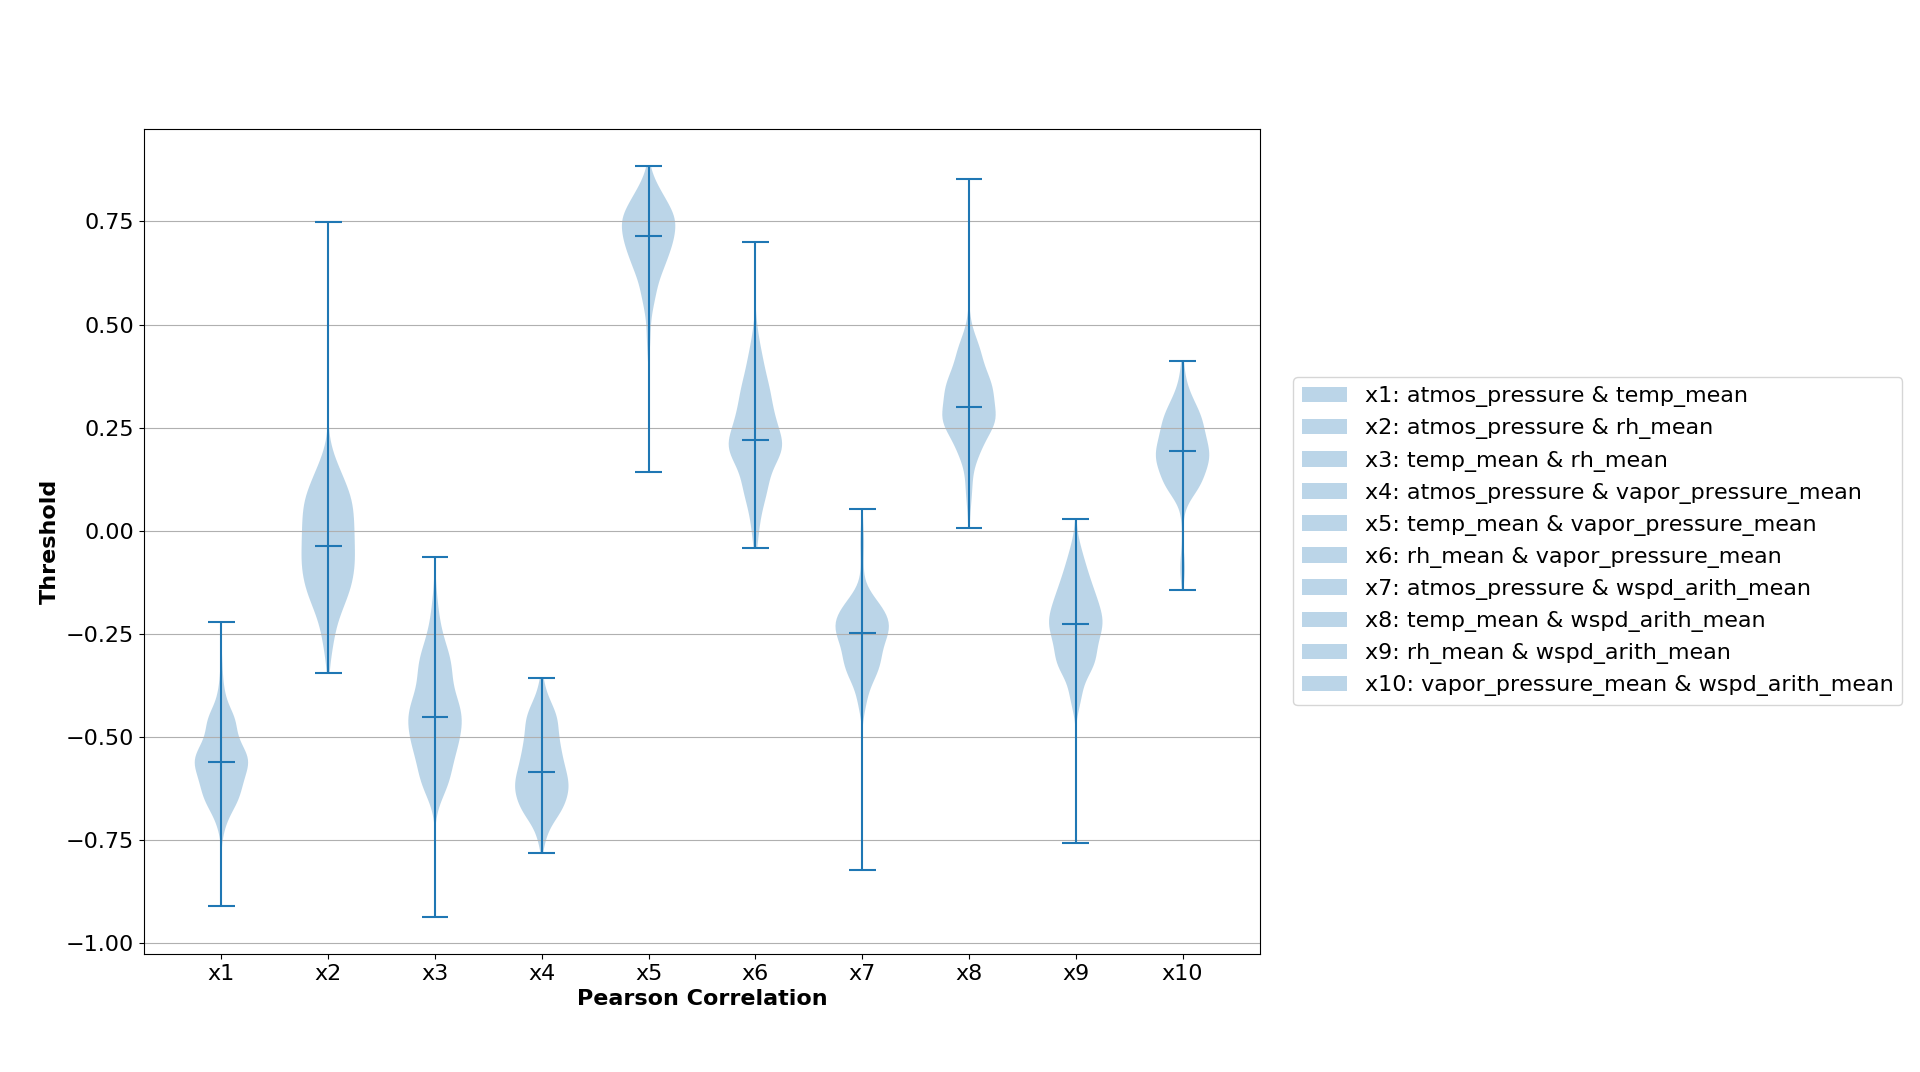
\includegraphics[width=\textwidth]{figures/Spring.png}
    \caption{Violin plot: Spring season, 5 variables from SGPMET}
    \label{fig:pc}
\end{figure*}

We performed a pairwise comparison of the five variables using Pearson
correlation using data from all 24 extended facilities. Atmospheric
dynamics are strongly driven by seasons and the correlation patterns
among meteorological variables can have season specific patterns. We
performed our analysis seasonally by separating the data among Winter, Spring,
Summer and Fall seasons. Figure~\ref{fig:pc} show the distribution of
pairwise correlation for Spring season. All variables show strong
correlations which are normally distributed. The long tails of the
distribution are potentially due to outlier data points. 
For example, the Pearson correlation between
\textit{temp\_mean} and \textit{vapor\_pressure\_mean} is positively
correlated with correlation mean close to 0.75. And the Pearson
correlation between \textit{atmos\_pressure} and \textit{temp\_mean} is
negatively correlated with correlation mean close to -0.60. These highly
correlated Pearson correlation coefficients are stored as the expected
values between two variables. We then compare each Pearson correlation
of two variables from a specific season in a specific year from a
specific instrument individually. If this pairwise Pearson correlation
of two variables deviates far away from our stored base knowledge, we
treat it as an outlier. We can also use this method to check whether the
upcoming data contains outliers.

\subsection{Singular Spectrum Analysis}
Singular Spectrum Analysis (SSA) is a popular method for time series
data analysis \cite{golyandina2013singular, golyandina2014basic}. The
general idea is to use a subset of the decomposition of trajectory
matrix to approximate the original data. Many applications can be found
in \cite{golyandina2013singular}. For example, SSA can be applied to
monitor volcanic activity \cite{bozzo2010relationship}. It can also be
used to extract trend \cite{alexandrov2008method}. Different from the
classic SSA method, we defined our own version of SSA which is designed
to remove any number of modes of specified periodicity from the time
series. This is meant to remove known seasonalities from the data in 
order to isolate true anomalous values more accurately. We provided a 
schematic of the algorithm used in Figure~\ref{fig:pcs} and a sample 
application in Figure~\ref{fig:ssa}.

% SSA workflow
\begin{figure}[ht]
    \centering
    % Define block styles
    \tikzstyle{decision} = [diamond, draw, fill=blue!20, text width=4.5em,text badly centered, node distance=3cm, inner sep=0pt]
    \tikzstyle{block} = [rectangle, draw, fill=blue!20, minimum width=5em, text centered, rounded corners, minimum height=2em]
    \tikzstyle{line} = [draw, -latex']
    \tikzstyle{cloud} = [draw, ellipse,fill=red!20, node distance=3cm, text width=3em, minimum height=2em]
    \begin{tikzpicture}[node distance = 2cm, auto]
        % Place nodes
        \node [block] (init) {\small Embedding};
        \node [block, right of=init, node distance=3cm] (decomp) {\small Decomposition};
        \node [block, below of=decomp] (freq) {\small Finding Dominant Frequency};
        \node [block, below of=freq] (period) {\small Converting Periodicity into Frequency};
        \node [block, below of=period] (approx) {\small Approximation};
        \node [block, left of=approx, node distance=3cm] (re) {\small Reconstruction};
        % Draw edges
        \path [line] (init) -- (decomp);
        \path [line] (decomp) -- (freq);
        \path [line] (freq) -- (period);
        \path [line] (period) -- (approx);
        \path [line] (approx) -- (re);
    \end{tikzpicture}
    \caption{Flowchart of SSA}
    \label{fig:pcs}
\end{figure}

\begin{figure*}[ht]
    \centering
    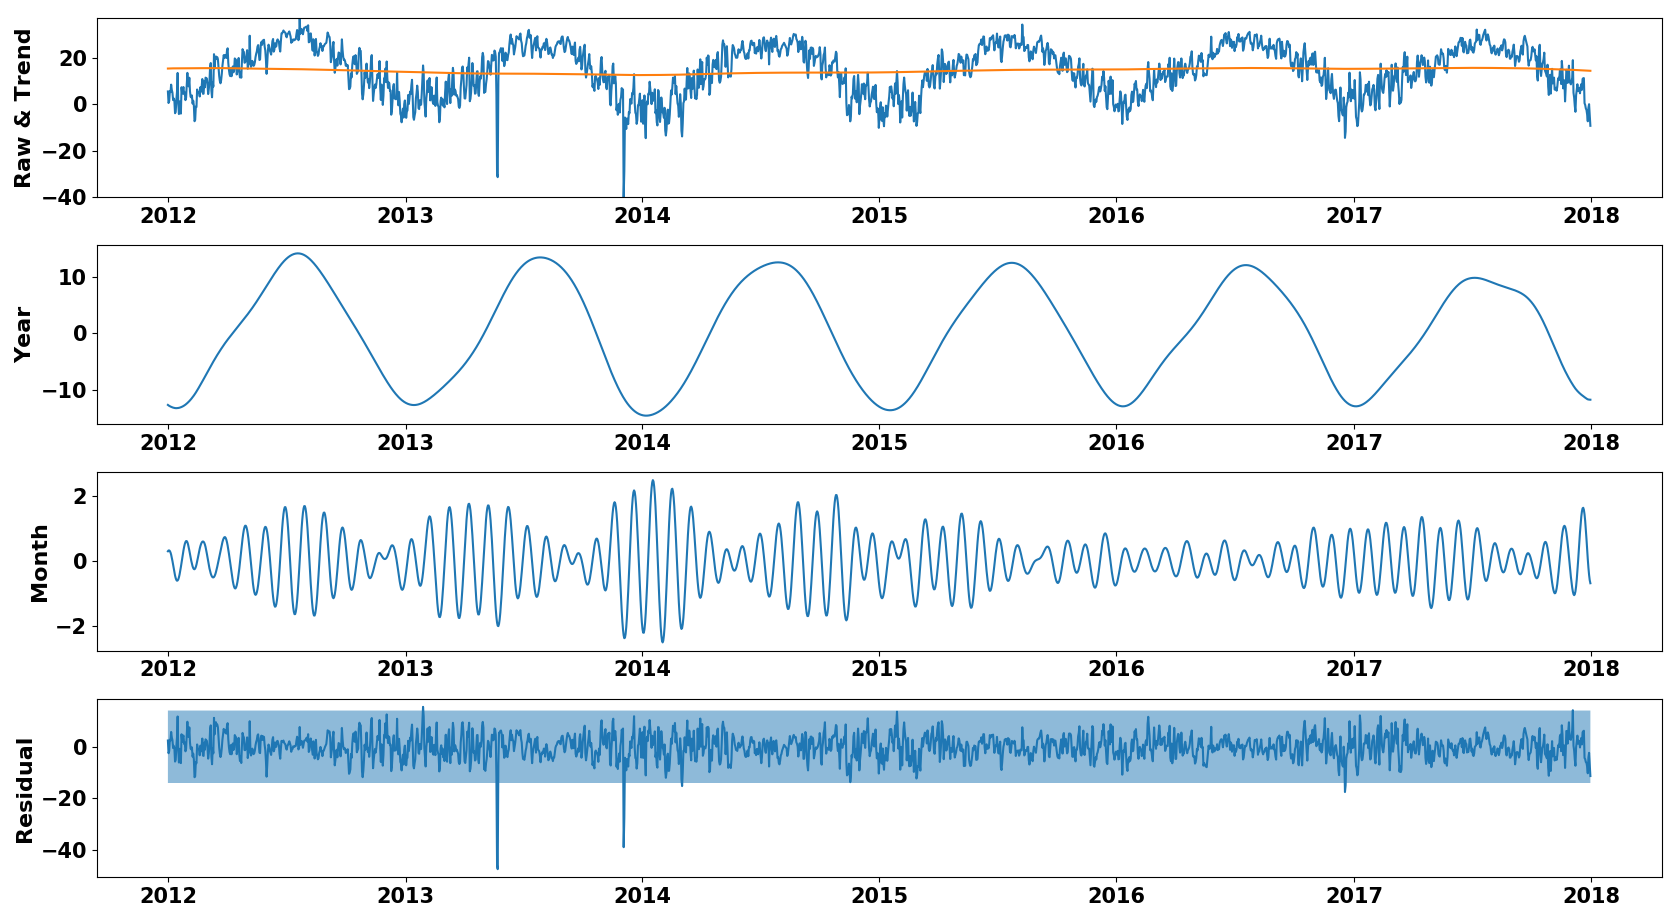
\includegraphics[width=\textwidth]{figures/E33.png}
    \caption{Example of SSA application on ARM data. The full decomposition of \textit{temp\_mean} data from MET instrument deployed in facility E33.}
    \label{fig:ssa}
\end{figure*}

% SSA algorithm description
Assume we have an ARM time series data Y of length T
\begin{align*}
Y =(y_1,\ \ldots,\ y_T)
\end{align*}
where $T > 2$ and $y_i$ is not empty. Let $L\ (1 < L \leq T/2)$ be the window size and $K = T - L + 1$. In general, the algorithm contains two main parts: decomposition and reconstruction. The first step is to form the trajectory matrix \textbf{X} from vector Y by embedding subsets of Y. These subsets of Y $X_i$ are lagged vectors of length L.  
\begin{align*}
X_i = (y_i,\ \ldots,\ y_{L+i-1})^T \quad (1 \leq i \leq K) \\
\mathbf{X} = [X_1,\ \ldots,\ X_K] 
\end{align*}
Thus the trajectory matrix is
\begin{equation}
\mathbf{X} = (x_{ij})_{i,j=1}^{L,K}  = \left(\begin{IEEEeqnarraybox*}[][c]{,c/c/c/c/c,}
y_1 & y_2 & y_3 & \ldots & y_K\\
y_2 & y_3 & y_4 & \ldots & y_{K+1}\\
y_3 & y_4 & y_5 & \ldots & y_{K+2}\\
\vdots & \vdots & \vdots & \ddots & \vdots\\
y_L & y_{L+1} & y_{L+2} & \ldots & y_T
\end{IEEEeqnarraybox*}\right)\label{e:traj}
\end{equation}
where $x_{ij} = y_{i+j-1}$. We can see from equation 1 that matrix \textbf{X} has equal elements on anti-diagonals and therefore it is a Hankel matrix. Then we perform the singular value decomposition (SVD) on $\mathbf{S}=\mathbf{XX}^T$ where the eigenvalues of S are denoted by $\lambda_1, \ldots, \lambda_L$ in the decreasing order of magnitude $(\lambda_1 \geq \ldots \geq \lambda_L \geq 0)$ and the corresponding eigenvectors by $P_1, \ldots, P_L$. Let $d = rank\ \mathbf{X}$ and $V_i = \mathbf{X}^T P_i / \sqrt{\lambda_i} (i = 1, \ldots, d)$. Thus, the trajectory matrix X can then be written by its eigendecomposition,
\begin{equation}
\mathbf{X} = \mathbf{X_1} + \ldots + \mathbf{X_d}
\end{equation}
where $\mathbf{X_i} = \sqrt{\lambda_i} P_i V_i^T$.

Next we choose a subset of eigenpairs to form an approximation of the
trajectory matrix. It is at this point that our version of the algorithm
differs. Given that the time series we are studying has seasonality at
known frequencies, we use Fast Fourier transform (FFT) to find the
dominant frequency of each eigenvector \cite{cooley1965algorithm}. We
then approximate the trajectory matrix by including modes which match
the frequencies of the seasonality we wish to remove. For example, we
anticipate that the temperature data will have a annual and possibly
monthly cycle, as shown in Figure~\ref{fig:ssa}. SSA allows us to tease
out these contributions in additive fashion. In this example, the
signals from the year, month, and residual sum together to form the
original raw data. This residual is then the noise in the raw data with
the seasonality removed as doing so exposes large anomalies which are
possible outliers. %Algorithm 1 shows the whole process.

%\begin{algorithm}[ht]
%\DontPrintSemicolon
%\SetAlgoLined
%%\KwResult{Dominant frequency of each eigenvector}
%\SetKwInOut{Input}{Input}
%\SetKwInOut{Output}{Output}https://v2.overleaf.com/9723918617khctmsbmkbqg
%\Input{$\lambda$ of $\mathbf{S}$ and corresponding eigenvectors $\mathbf{P}$}
%\Output{Dominant frequency of each eigenvector}
%\BlankLine
%
%fftfreq $\leftarrow$ Discrete Fourier Transform sample frequencies\;
%fft $\leftarrow$ Discrete Fourier Transform\;
%len $\leftarrow$ size of $\lambda$\;
%frequencies $\leftarrow$ zero vector of size len\;
%fs $\leftarrow$ fftfreq($\lambda$)\;
%ix $\leftarrow$ indices that sort fs\;
%fs $\leftarrow$ fs[ix]\;
%\For{i in range(len)}{
%    p1 $\leftarrow$ abs(fft($\mathbf{P}$[:,i]))\;
%    ps $\leftarrow$ p1**2\;
%    ps $\leftarrow$ ps[ix]\;
%    frequencies[i] $\leftarrow$ fs[index of the maximum value in ps]\;
%}
%\Return abs(frequencies)
%\caption{Dominant Frequency Finder}
%\end{algorithm}

Once the eigenpairs are chosen, we proceed with the classical definition
of the method. If $I$ represents a set of indices corresponding to the
eigenmodes to remove, we approximate the trajectory matrix
%
\begin{equation*}
    \mathbf{Xt} = \sum_{i\in I} \mathbf{X_i}
\end{equation*}
%
An approximation $Yt$ to the original signal $Y$ can be obtained from
$\mathbf{Xt}$ by inverting the process used to form the trajectory
matrix, Equation~\eqref{e:traj}. Each column of $\mathbf{Xt}$ represents
a shifted approximation to $Yt$, thus we average each shifted column.
Finally the deseasonalized residual is the difference between the
original signal and the reconstruction, $R=Y-Yt$.

In this paper, we chose the \textit{temp\_mean} data from instrument E33
as $Y$ to illustrate SSA. Because SSA requires the time series data to
be continuous, we replaced the empty points with the average temp\_mean
value for that day in a year. We set $L = 400$ and picked a single year
and month as the periodicity groups. Thus $Yt = Yt[0] + Yt[1] + Yt[2]$.
Figure~ \ref{fig:ssa} is a visualization of the result. The first row is
the raw data $Y$. The orange line $Yt[0]$ is the trend. As we can see
from the figure, the trend is pretty flat from 2012 to 2017. The second
row and third row are $Yt[1]$, $Yt[2]$ respectively. The Year data
matches the pattern of the raw data. The last row is the residual. Those
peak values outside the blue shaded area are outliers.

\subsection{K-means}
K-means is a partitioning clustering algorithm \cite{macqueen1967some,
hartigan1979algorithm}. It starts with the k centroids user
specified, and assigns the points to the nearest centroid. Then it
computes new k centroids and assign the rest points to these
centroids again. The process repeats until it converges. 

% K-means algorithm
\begin{algorithm}[ht]
\DontPrintSemicolon
\SetAlgoLined
%\KwResult{Dominant frequency of each eigenvector}
\SetKwInOut{Input}{Input}
\SetKwInOut{Output}{Output}
\Input{ARM time series data}
\Output{Outliers}
\BlankLine

outliers $\leftarrow \varnothing$\;
df $\leftarrow$ ARM time series data\;
data $\leftarrow$ df[`atmos\_pressure',`temp\_mean',\
`rh\_mean',`vapor\_pressure\_mean',`wspd\_arith\_mean']\;
number\_of\_clusters $\leftarrow$ 4\;
clusters $\leftarrow$ K-means(data, number\_of\_clusters)\;
distances $\leftarrow$ Distance between each point and its centroid\;
mean $\leftarrow$ arithmetic mean of distances\;
sigma $\leftarrow$ standard deviation of distances\;
threshold $\leftarrow$ mean + 3 * sigma\;
\For{i in range(size of distances)}{
    \If{distances[i] $>$ threshold}{
        outliers $\leftarrow$ outliers $\cup$ {distances[i]}
    }
}
\Return outliers
\caption{K-means Outlier Detection}\label{alg:kmeans}
\end{algorithm}

In this paper, we did not stop after clustering ARM data with K-means.
We transformed the generated clusters into a vector of distance between
each point and its corresponding centroid. If the distance of a point is
larger than the threshold, this point will be filtered out as an
outlier. Algorithm~\ref{alg:kmeans} describes the whole process. Unlike
SSA, we used all the 5 variables mentioned in Datasets section together
to extract outliers.

\begin{figure*}[ht]
    \centering
    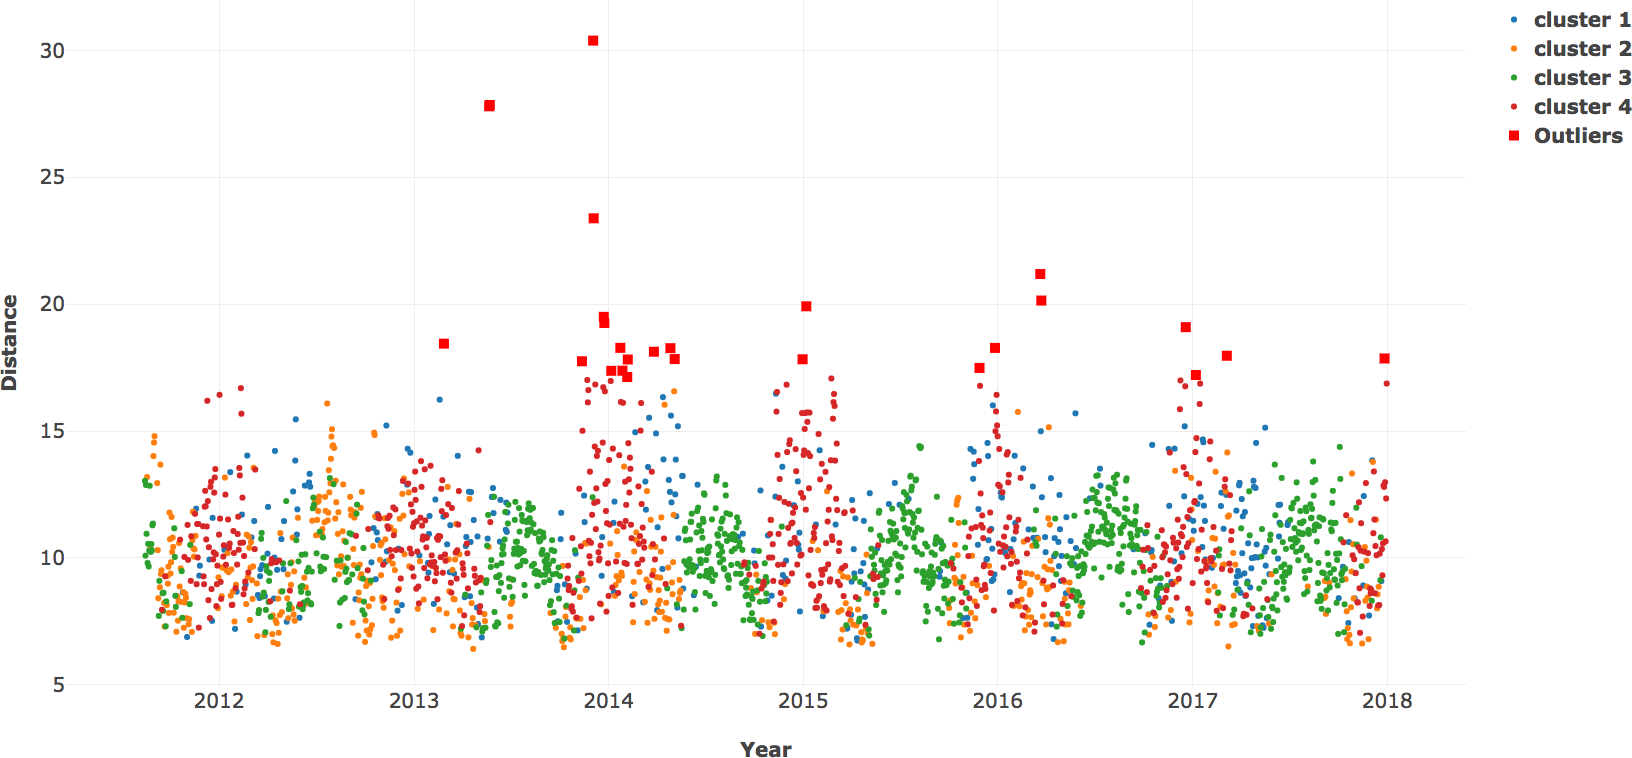
\includegraphics[width=\textwidth]{figures/kmeans.png}
    \caption{Outliers detected using K-means for E33}
    \label{fig:kmeans}
\end{figure*}

Again, we used data from instrument E33 as an example for K-means. Here
we set k to 4 as each year has 4 seasons.  Figure~\ref{fig:kmeans}
visualized the outliers detected from E33. Y axes in this figure is the
distance metric. Those red squares which are far away from the centroids
are outliers.




%% Results and discussions
\section{Results and Discussion}
% mention the usage of python and implementation. % add three sigma rule here.
The three algorithms and visualizations presented in this paper are 
implemented in Python. All codes and results are available on GitHub 
(https://github.com/YupingLu/arm-pearson and https://github.com/YupingLu/arm-ssa). 
Multiple methods are available to set a threshold for extreme values as 
outliers. We used the three sigma rule to extract outliers \cite{pukelsheim1994three}. 
For example, if the distance of one point is larger than three sigmas, 
we treat this point as an outlier in Algorithm~\ref{alg:kmeans}.

% methods drawbacks and advantages
Pearson correlation coefficient is a pairwise comparison method which 
is used to detect abnormality of correlation between two variables. 
However if the two variables suddenly change in the same direction, 
their correlation may still be normal similar to their ``supposed" 
value. It is the same case if only a few points are outliers as the
correlation is determined by the majority of data points. 
As we performed the Pearson correlation 
coefficient on the seasonal level, it is not possible to track down 
to the exact day. SSA is a univariate method to detect outliers for 
each variable in the ARM data. It can quickly catch those high peak 
and drop points. But it requires the time series data to be continuous 
with no missing values. K-means is a commonly used multivariate method 
for clustering. Here we used it for outlier detection. The drawback of this method is 
that the detected outliers could be just one type of variable or 
multiple types of variable. It is hard to tell which is the case for 
corrected the new data. As we also averaged the raw 
minute level data into day level data, some outliers may be averaged 
out by this process.

% all together as a template
One outlier may only be detected by SSA or Pearson correlation coefficient 
or K-means. Thus we combined all the three methods together as a 
whole framework. SSA and K-means are used to detect outliers whereas Pearson 
correlation coefficient can be used to detect the variables causing the anomaly 
in the K-means results by using the pairwise correlations. Figure~\ref{fig:combined} is the result of 
detected outliers for \textit{temp\_mean} from E33. The red squares 
stand for the common outliers detected by both K-means and SSA. The 
orange diamonds are the ones detected by K-means excluding the common 
outliers. And the black stars represents the outliers detected by SSA 
excluding the common outliers. We can see from the figure that more 
outliers have been detected compared to Figure~\ref{fig:ssa} and Figure~\ref{fig:kmeans}. 
Thus we applied this framework on all the test data. Table~\ref{tab:comp} 
shows the number of detected outliers. The size of common detected 
outliers is 378 by this framework.

\begin{figure*}[ht]
    \centering
    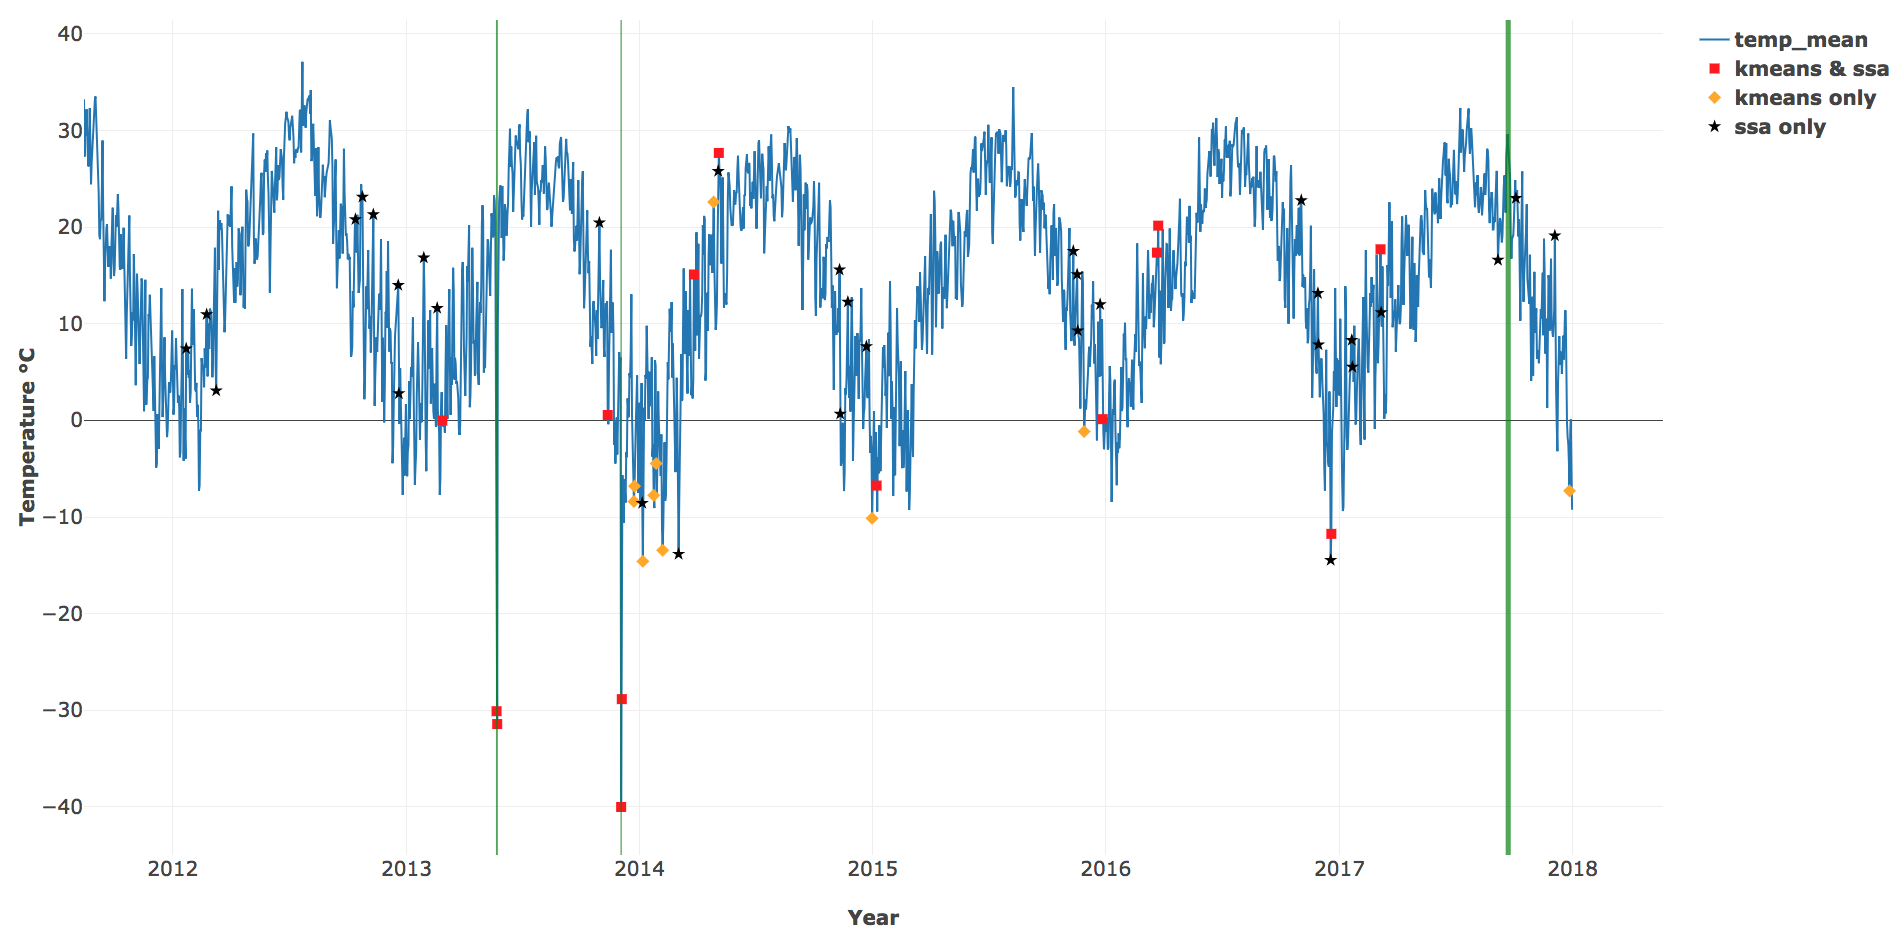
\includegraphics[width=\textwidth]{figures/combined.png}
    \caption{Outliers detected for E33 \textit{temp\_mean} using combined algorithms}
    \label{fig:combined}
\end{figure*}

\begin{table}[ht]
\caption{Comparison of SSA and K-means Outlier Set Size}
\label{tab:comp}
\centering
\begin{tabular}{|l|c|}
\cline{2-2}
\multicolumn{1}{l|}{} & Outlier Set Size\\
\hline
SSA & 922\\
K-means & 508\\
Intersection & 378\\
Symmetric Difference & 674\\
\hline
\end{tabular}
\end{table}

\begin{table}[ht]
\caption{Precision and Recall of SSA and K-means}
\label{tab:pr}
\centering
\begin{tabular}{|l|c|c|c|}
\hline
Method & Variable & Precision & Recall\\
\hline
SSA & temp\_mean & 16.00\% & 1.20\%\\
SSA & vapor\_pressure\_mean & 20.70\% & 1.40\%\\
SSA & atmos\_pressure & 0.00\% & 0.00\%\\
SSA & rh\_mean & 14.80\% & 0.50\%\\
SSA & wspd\_arith\_mean & 0.60\% & 1.50\%\\
Kmeans & 5 together & 12.90\% & 1.90\%\\
Combined & 5 together & 11.10\% & 4.10\%\\
\hline
\end{tabular}
\end{table}

% DQR here
The current data quality or outlier detection is maintained as data 
quality reports (DQRs) stored in the DQR database with each entered 
manually \cite{mccord2016arm}. A description of an event which 
changed the normal data is included in these DQRs. The event could 
be temporary operating conditions such as power failures, frozen 
and snow covered sensors, instrument degradation, or contamination. 
It could also be an extreme weather event that has never been observed 
before. Each DQR entry also contains a specific time range affected, 
list of data projects, and specific measurements. And these entries 
are usually submitted by either the Data Quality Office \cite{peppler2016arm} 
or the instrument mentor \cite{cress2016deploying}. It is easy to 
notice that this method is not efficient as it requires a lot of labor. 
It is also nearly impossible to detect all the outliers due to the 
complexity and high volume of the ARM data.

Currently, not many outliers entries are stored in DQR database. Here we 
used manually detected 181 outliers in the DQR database as the ground 
truth to compare with the results from our framework. Precision and 
recall which were first defined in \cite{perry1955machine} were used 
as the comparison metric. They are commonly used to measure the quality 
of classification tasks \cite{olson2008advanced}. Precision is calculated 
as True Positives divided by the sum of True Positives and False 
Positives. On the other hand, recall is measured from True Positives 
divided by the sum of True Positives and False Negatives. We treated 
outliers in DQR database as True Positives. Thus detected outliers not 
in the DQR database are False Positives. Undetected values which in 
the DQR database are False Negatives, and which not in the DQR database 
are True Negatives. Table~\ref{tab:pr} contains the statistics of 
the comparison.

Precision attempts to answer the proportion of positive identifications that
was actually correct. The Combined precision is 11.10\% which shows that 
many outliers detected by the framework are not in the DQR database. 
Recall tries to solve the proportion of actual positives identified 
correctly. The number is 4.10\% which is even smaller than precision. 
One reason for small recall is that the size of True Positives 
is much small. The other reason is that DQR database records the whole 
possible affected time range which makes the size of False Negatives 
large. It could be possible that only a few days of the data recorded 
during that time range are actually outliers.



%% Conclusions
\section{Conclusions}
In this paper we tested pairwise Pearson correlation,
univariate SSA and multivariate $k$-means based method for detection of
outliers in the data at ARM meteorological observations at SGP site. 
Combining the approaches within a framework for
streaming data within ARM provides a platform to detect outliers
from a wide range of sensor failure scenarios to extreme events.
While each of the methods developed and applied in this study has its
strengths and limitations, our evaluation against existing database of
data quality issue suggests that the framework is able to identify known
outliers well. Although our current study focused on
meteorological observations, it provides a framework for an efficient
outlier detection of streaming datasets within ARM that can be extended to
other classes of time series datasets not only tested MET data from SGP. 
In the future, we plan to analyze multiple
classes of instruments like meteorological, radiometric, radar etc.
simultaneously for improved detection of outliers. We also plan to
develop multivariate SSA \cite{rodrigues2018benefits} and machine learning 
techniques to address this high dimensional problem in an operational 
data center environment.

The three algorithms and visualizations presented in this paper are 
implemented in Python. All codes and results are available on GitHub 
(https://github.com/YupingLu/arm-pearson and https://github.com/YupingLu/arm-ssa). 


\section*{Acknowledgment}
This research was supported by the Atmospheric Radiation Measurement (ARM) user 
facility, a U.S. Department of Energy (DOE) Office of Science user facility 
managed by the Office of Biological and Environmental Research.


\bibliography{references} 
\bibliographystyle{IEEEtran}


\end{document}
